%% Aggregate Accuracy Does Not Reveal Reliability -- ISPRS Journal of Photogrammetry and Remote Sensing (Elsevier)
%% Compile on Overleaf (has elsarticle + natbib) or locally with: latexmk -pdf main.tex
%% Figures fig2_flagship_reliability.pdf and fig3_domain_gaps.pdf must be in the same directory.
\documentclass[preprint,3p,times]{elsarticle}

\usepackage{amsmath,amssymb}
\usepackage{graphicx}
\usepackage{booktabs}
\usepackage[hidelinks]{hyperref}
\usepackage{textcomp}
\setlength{\emergencystretch}{2em}   % absorb the few minor overfull lines gracefully

\journal{ISPRS Journal of Photogrammetry and Remote Sensing}

\begin{document}

\begin{frontmatter}

\title{Aggregate Accuracy Does Not Reveal Reliability: Silent Conformal Certificate Failure from a Stale Preprocessing Contract under Operational Spectral and Domain Shift in Sentinel-2 Cloud Segmentation}

\author[a]{Hsiu-Chi Tsai\corref{cor1}}
\ead{hctsai1006@cs.nctu.edu.tw}
\author[b]{Chia-Tung Chung}
\ead{jun.514114.ee10@nycu.edu.tw}
\cortext[cor1]{Corresponding author.}
\affiliation[a]{organization={Arete Honors Program, National Yang Ming Chiao Tung University}, addressline={No.~1001, University Road, East District}, postcode={300093}, city={Hsinchu City}, country={Taiwan}}
\affiliation[b]{organization={Department of Photonics, National Yang Ming Chiao Tung University}, addressline={No.~1001, University Road, East District}, postcode={300093}, city={Hsinchu City}, country={Taiwan}}

\begin{abstract}
Operational Earth-observation pipelines increasingly gate downstream decisions on deep segmentation outputs, and a large literature measures how well their \emph{accuracy} survives distribution shift. We show that accuracy-robustness is not enough: a conformal certificate calibrated before deployment and reused under shift can fail \emph{silently}. Using split conformal risk control on Sentinel-2 cloud segmentation (CloudSEN12) under the operational L1C$\to$L2A atmospheric-correction shift, pixel accuracy falls $12$ points ($79.6 \to 67.9\,\%$) while a clean-calibrated threshold's confidently-wrong (joint) risk more than triples, $8.5 \to 27.8 \pm 0.8\,\%$ against a $10\,\%$ target---a rise the calibration statistic it minimises never reports (it stays below target by construction), masking a per-class collapse in the minority cloud classes. We trace the breach primarily to a \emph{stale input-normalization contract}: the model standardizes L2A with its L1C training statistics. Re-normalizing the deployment input with target-product-state statistics, estimated from an unlabelled target calibration sample, returns the joint risk toward target---product-aware standardization reaches $10.8\,\%$ and a fuller per-band quantile transport $9.6\,\%$ (interval $[9.0,10.1]$), at clean-like coverage and without target labels---so the dominant effect is a preprocessing-and-certificate contract mismatch under a metadata-visible product change, not a general law that atmospheric correction destroys conformal reliability. The failure is not an artefact of one processor, scene set, or operating point: a second, algorithmically distinct processor (ACOLITE) breaks the same certificate equivalently ($29.6\,\%$; paired difference $+0.26$, two one-sided tests passing a $\pm2\,\%$ margin), it replicates on the official held-out validation scenes ($28.0\,\%$; a within-dataset held-out replication), and it persists for targets from $5$ to $20\,\%$. Covariate-shift weighted conformal does not restore a \emph{useful} certificate: source-only reweighting over-accepts, while a formal plug-in estimated-weight control holds the joint risk valid only by abstaining to $7\,\%$ coverage---operationally useless, not invalid---because clean and L2A are near-separable (AUROC $0.99$)---poor overlap, which a matched control attributes to lack of overlap, not weight mis-estimation (and the plug-in weight inherits no exact finite-sample guarantee). The severity is also conditional and model-specific: a structural surface-brightness gap gives a suggestive but inferentially inconclusive excess ($11.3\,\%$), a milder geographic gap shows no clear evidence of a breach ($9.7\,\%$), a channel-adaptive foundation model (DOFA) is far more reliable ($9.9\,\%$), and within a matched convolutional family a larger receptive field attenuates the breach. We report every risk with its coverage---a joint mass that abstention alone can drive to zero---and certify against a scene-connected-component exchangeable unit with two-way cluster-robust standard errors. To our knowledge this is the first demonstration of silent conformal-certificate failure for Sentinel-2 optical segmentation under a real atmospheric-correction shift, traced to a stale preprocessing contract rather than to atmospheric physics alone.
\end{abstract}

\begin{keyword}
conformal prediction \sep uncertainty quantification \sep distribution shift \sep cloud segmentation \sep Sentinel-2 \sep operational reliability
\end{keyword}

\end{frontmatter}

\section{Introduction}
Earth-observation segmentation models are moving from research benchmarks into operational pipelines: cloud masking that gates every downstream surface-reflectance product, land-cover mapping that feeds policy, change detection that triggers alerts. In these settings the model rarely sees the exact distribution it was trained on. The Sentinel-2 archive alone exposes a model to at least four operational shifts: the L1C$\to$L2A atmospheric correction that transforms top-of-atmosphere reflectance to bottom-of-atmosphere reflectance and removes the cirrus band B10; cross-sensor transfer as constellations evolve; deployment across geographies and seasons absent from the training set; and deployment on surface types (bright built-up, bare soil, snow and ice) that are both operationally critical for cloud confusion and under-represented in labelled data.

A substantial literature now measures how well models \emph{maintain accuracy} under such shifts. Channel- and sensor-adaptive encoders \citep{xiong2024dofa,waldmann2025panopticon,francis2021sensei,bao2024channelvit} are evaluated on their cross-band and cross-sensor accuracy; robustness benchmarks score accuracy under image-space corruptions \citep{li2025reobench}; cross-band generalisation studies quantify accuracy transfer across spectral-band configurations \citep{tamazyan2025geocrossbench}. What this literature does not ask is whether, \emph{under the same shifts}, the model still \textbf{knows when it is wrong}---whether the uncertainty it reports remains trustworthy. That question is not a refinement of accuracy-robustness; the two can decouple. A model can preserve its mean accuracy while its confidence-to-error relationship silently drifts, so that a fixed operating point calibrated before deployment admits far more confident errors than it certifies.

Conformal prediction offers a principled way to \emph{certify} such an operating point: split conformal and its risk-controlling variants give a finite-sample guarantee on a chosen error notion. But the guarantee holds only under exchangeability between calibration and test data, and operational shift is precisely a controlled violation of exchangeability. The danger is not that the certificate fails loudly---it is that it fails \emph{silently}: the calibration-set statistic the procedure minimises stays below target by construction, so a practitioner reading only that number sees success, while the deployed risk runs above target with nothing to announce it.

This paper makes that failure concrete, operational, and---crucially---bounded. Our contributions are:
\begin{itemize}
\item \textbf{C1 --- Reliability degrades disproportionately to accuracy, and silently, under a real atmospheric shift.} On CloudSEN12, under the genuine L1C$\to$L2A Sen2Cor transition (not a synthetic ablation), pixel accuracy falls 12 points while a clean-calibrated conformal threshold's confidently-wrong joint risk more than triples to $27.8\,\%$ against a $10\,\%$ target. The reliability breach is disproportionate to the accuracy loss and is never announced, since the certificate's own calibration statistic still passes (Section~\ref{sec:flagship}).
\item \textbf{C2 --- In the shifts we test, whether a breach appears differs by the kind of shift, and severity is model-specific.} Two pure deployment shifts (input held fixed) separate the conditions: a structural surface gap produces a suggestive excess above target ($11.3\,\%$, significant under the two-way SE but inconclusive under the full nested calibration-resampling bootstrap), while a milder geographic gap gives no clear evidence of a breach ($9.7\,\%$, close to target). With only these two hand-chosen splits---which also co-vary class prevalence, season, biome and calibration size---and no independently-measured domain-gap metric, we read this as an illustrative contrast between two deployment shifts, not a general law that shift kind determines whether a breach occurs, and not a claim that severity tracks a measured gap size. The severity is also model-specific: within a matched convolutional family, a larger receptive field modestly attenuates the breach (raw kernel sweep $1\times1$ $20.4\,\% \to 7\times7$ $17.4\,\%$; the attenuation survives parameter-matched controls at receptive fields ${\geq}17$px), and a channel-adaptive foundation model (DOFA) is far more reliable ($9.9\,\%$), so the crisis is softened across the tested models rather than universal---though we attribute no fixed point count to spatial context or pretraining across architectures (Sections~\ref{sec:deployment}--\ref{sec:modelclass}).
\item \textbf{C3 --- The dominant mechanism is a stale normalization contract, and the first remedy needs no labels.} We trace the atmospheric breach to a stale input-normalization contract---the model standardizes every product with its source (L1C) training statistics and reuses them on L2A---and show that re-normalizing the deployment input with unlabelled target-domain calibration-sample statistics reduces the \emph{empirical} risk toward the target level (product-aware standardization to $10.8\,\%$, its interval just above $10\,\%$; a richer per-band quantile transport to $9.6\,\%$, its interval straddling $10\,\%$) at clean-like coverage, without target labels or abstention---an empirical reduction on the deployment scenes, not a re-derived finite-sample guarantee, because the transform is estimated from deployment data and no longer satisfies the source split's exchangeability (Section~\ref{sec:flagship}). Where a residual remains or the shift is not a normalization change (the surface gap), per-stratum (Mondrian) recalibration on target-state labels is a second, costlier remedy; because the certified quantity is a joint mass that abstention alone can drive to zero, we report every risk with its coverage and quantify the coverage each remedy spends.
\item \textbf{C4 --- The methodology a defensible certificate on this data requires.} The exchangeable unit must be the scene-connected component, not the annotation ROI---12 Sentinel-2 products in the CloudSEN12 test split each appear under two ROIs, so ROI-level splitting leaks a scene across calibration and test---and the standard error over the crossed calibration-split $\times$ model-seed design must be two-way cluster-robust rather than treating the 100 cells as independent (Section~\ref{sec:method}).
\end{itemize}

We are deliberate about scope. We claim only the \emph{operational instantiation}: that a naive conformal certificate can lose its validity under distribution shift is established theory (the coverage-gap bound of \citet{barber2023}, and the online treatment of \citet{gibbs2021}), with weighted conformal a known remedy under known covariate shift \citep{tibshirani2019}; the risk-control machinery is borrowed \citep{angelopoulos2024}; per-stratum recalibration is a Mondrian special case \citep{vovk2005}; and the label-free repair we find is a known test-time-normalization remedy \citep{schneider2020,tent2021,dua2022,corley2024}, applied here to the input rather than to internal batch statistics. Our mechanism components (band-group tokenisation, wavelength-conditioned attention, spectral-group masked pretraining, band-group dropout) are cited reused ingredients, not claimed contributions. What is new is the demonstration, diagnosis and honest costing of this \emph{silent} certificate failure for operational remote-sensing segmentation on real Sentinel-2---that a routine calibration-to-deployment product-normalization mismatch silently invalidates the certificate while its own statistic still passes, and that a label-free product-aware re-normalization brings its empirical risk back near target (without re-deriving the finite-sample guarantee)---together with the exchangeability and variance methodology that makes the demonstration defensible.

\section{Related work}
\paragraph{Conformal prediction under distribution shift.} Split conformal prediction gives distribution-free finite-sample coverage under exchangeability; when calibration and test distributions differ, coverage is no longer guaranteed. Weighted conformal prediction \citep{tibshirani2019} recovers validity under \emph{known} covariate shift; \citet{barber2023} bound the coverage gap under general non-exchangeability; \citet{gibbs2021} and \citet{podkopaev2021} treat online and label shift, and \citet{cauchois2024} give distributionally-robust coverage over a bounded shift set. Conformal risk control \citep{angelopoulos2024} generalises coverage to monotone risks and is the machinery we adopt. Where coverage deviation under shift has been examined in a hyperspectral Raman-imaging setting it has been treated as an \emph{observable}, label-dependent diagnostic \citep{booksh2025}---the opposite of the silent failure we characterise here, in which the certificate's own statistic never signals the breach. We use none of these to \emph{fix} the shift---our naive arm is deliberately an unweighted certificate, so that its failure is the measurement; the remedy we study is the simplest valid instance, per-stratum (Mondrian, \citealt{vovk2005}) recalibration on discrete operational states.

\paragraph{Conformal and selective prediction in remote sensing.} Conformal methods have reached remote sensing, most often \emph{in distribution}: split-conformal hyperspectral classification with a within-scene permutation-invariance assumption to repair exchangeability \citep[SACP,][]{liu2024sacp}, and conformal \emph{risk} control for semantic segmentation---including the LoveDA aerial benchmark---with image-level exchangeability and no deployment shift \citep{mossina2024}. A smaller, largely concurrent line takes conformal or selective prediction to \emph{operational} shifts: out-of-calibration detection on scene classification under simulated corruption \citep{bhattacharjee2024}, spatial-covariate-shift conformal regression for satellite-derived air quality that measures coverage collapse \citep{adjei2026}, and out-of-distribution-triggered selective abstention in Earth-observation foundation models \citep{shrugfm2025}, and conformal prediction for Sentinel-2 flood segmentation \citep{floodconformal2025}. Our work differs from all of these in the three respects that define an operational reliability claim: it measures what happens to the conformal \emph{certificate itself} under a real atmospheric-correction (L1C$\to$L2A) shift on optical Sentinel-2 segmentation, rather than assuming exchangeability or testing a synthetic corruption; it makes the \emph{scene-connected component} the exchangeable unit, because pixel- and image-level exchangeability are broken by intra-scene correlation and by the shift; and its contribution is the \emph{measurement of certificate failure}---the robustness $\neq$ reliability decoupling---not the in-distribution production of prediction sets.

\paragraph{Robustness $\neq$ reliability.} The decoupling of accuracy-robustness from uncertainty-reliability has been observed outside remote sensing---under natural and medical distribution shift, chiefly through calibration and expected-calibration-error rather than conformal risk \citep{roschewitz2025,ovadia2019}. We give what is, to our knowledge, the first measurement of this decoupling for a conformal \emph{certificate} under a real atmospheric-correction shift in remote sensing.

\paragraph{Channel-adaptive and missing-band remote sensing.} Sensor- and channel-adaptive encoders \citep{xiong2024dofa,waldmann2025panopticon,francis2021sensei} and channel-sampling regularisers \citep{bao2024channelvit,pham2024dichavit} target \emph{accuracy} under varying or missing bands. We engage this literature as the source of our (cited) mechanism components and, in a companion decomposition (detailed in Appendix~\ref{app:companion} and released with the code), by showing which ingredients actually carry missing-band robustness and how that carrying is itself regime-dependent.

\section{Method}
\label{sec:method}
\subsection{Task, data, and models}
We study per-pixel cloud segmentation on CloudSEN12 \citep{aybar2022cloudsen12}, a Sentinel-2 benchmark of expert-labelled cloud and cloud-shadow masks with co-registered L1C (top-of-atmosphere, 13 bands) and L2A (Sen2Cor bottom-of-atmosphere, 12 bands; B10 removed, \citealt{mainknorn2017sen2cor}) products for the identical pixels. We deliberately study per-pixel spectral segmentation without spatial context, so that the reliability signal we measure is spectral and not a function of spatial redundancy; a spatial-context foundation-model baseline is included in Section~\ref{sec:modelclass}. The classes are clear, thick cloud, thin cloud, and cloud shadow. We use the manually-annotated \emph{high}-quality tier of the original CloudSEN12 release (as opposed to its scribble and unlabelled tiers), which already provides the paired L1C/L2A products our design needs, with the exact scene manifest in the released code; a re-run on the extended CloudSEN12+ labels is a label-version sensitivity check we leave to future work.

Our primary model is a band-as-modality encoder: physically-grouped spectral bands are tokenised, given a wavelength-conditioned positional encoding, mixed by cross-band attention, and pretrained with a spectral-group masked autoencoder before supervised fine-tuning with band-group dropout. This architecture is not a contribution---every ingredient is a cited reused component---but a substrate on which to measure reliability; we include a plain multilayer-perceptron baseline (with and without band-group dropout) and, in Section~\ref{sec:modelclass}, a frozen channel-adaptive foundation model \citep[DOFA,][]{xiong2024dofa}.

\subsection{Reliability framework}
For a fixed trained model we score every test pixel $p$ by its maximum softmax probability $c_p$ after temperature scaling, and study the operating point---an acceptance threshold $\lambda$ (accept $p$ iff $c_p \geq \lambda$)---selected by split conformal \emph{risk} control (CRC, \citealt{angelopoulos2024}) at a target risk $\alpha = 10\,\%$. The exchangeable unit is the scene-connected component $i$ (Section~\ref{sec:unit}); writing $S_i$ for its pixels, $\hat{y}_p$ for the prediction and $y_p$ for the label, the per-unit loss is the within-component confidently-wrong fraction
\begin{equation}
L_i(\lambda) \;=\; \frac{1}{|S_i|}\sum_{p \in S_i} \mathbb{1}\!\left[\,c_p \geq \lambda \;\wedge\; \hat{y}_p \neq y_p\,\right].
\label{eq:loss}
\end{equation}
Over $n$ calibration components CRC selects the lowest threshold whose finite-sample calibration bound meets the target,
\begin{equation}
\hat{\lambda} \;=\; \inf\Big\{\lambda : \tfrac{n}{n+1}\,\hat{R}_n(\lambda) + \tfrac{B}{n+1} \leq \alpha\Big\}, \qquad \hat{R}_n(\lambda) = \tfrac{1}{n}\sum_{i=1}^{n} L_i(\lambda),
\label{eq:crc}
\end{equation}
with loss bound $B = 1$ (the per-pixel term is a $0/1$ indicator, so each $L_i \in [0,1]$ and $\sup L = 1$), searched over the grid of calibration confidence values augmented with $\lambda_{\max} = +\infty$---the only threshold that abstains on \emph{every} point, including test pixels whose confidence has shifted above the entire calibration range (no flagship naive run selected this abstain-all threshold; it is reached only near the conformal feasibility floor, e.g.\ the surface Mondrian arm). Under exchangeability of $L_1,\dots,L_{n+1}$ this certifies the \emph{joint} confidently-wrong mass
\begin{equation}
\mathbb{E}\!\left[L_{n+1}(\hat{\lambda})\right] \;=\; P(\text{accepted} \wedge \text{wrong}) \;\leq\; \alpha
\label{eq:guarantee}
\end{equation}
\citep[Thm.~2.1]{angelopoulos2024}: a \emph{marginal}, hierarchical expectation over the joint draw of calibration and test---a component drawn with equal weight and then, within it, its pixels; equivalently, the mean over a freshly drawn component of its within-component confidently-wrong fraction---not a per-run promise, so a single realisation may exceed $\alpha$ without contradicting it. Two properties of this estimand are load-bearing and we hold to them throughout. First, the certified quantity is a \emph{joint} mass, not the selective risk $P(\text{wrong} \mid \text{accepted})$; abstaining drives it to zero, so we always report it with its coverage $P(\text{accepted})$ and its selective risk, and within a single weighting $\text{joint} = \text{selective} \times \text{coverage}$ holds exactly. Second, the certified estimand is \emph{component-equal-weighted}---each component contributes $L_i$ with equal weight, which is what ``draw a fresh component'' means---and this differs from the pixel-pooled (sample-weighted) risk whenever components differ in size. We therefore fix the component-equal weighting for the entire certified triple (joint, coverage, selective risk) and never pair a risk computed under one weighting with a coverage computed under another; the segmentation accuracy we quote alongside is the standard pixel-level figure, which we keep distinct from the certified ratio rather than folding it in. We verify in Section~\ref{sec:flagship} that recomputing the certified triple pixel-pooled instead of component-equal leaves the headline essentially unchanged, so it does not hinge on this choice.

We contrast two arms at each shift state. The \textbf{naive} arm calibrates the threshold and temperature once, on the source (clean / in-training) distribution, and deploys them under shift. The \textbf{Mondrian} arm recalibrates the threshold and temperature on the shifted (target) state itself. The strata are pre-defined operational states (product level, surface class, hemisphere), fixed before any evaluation rather than chosen after seeing results. A third \textbf{control} arm (source threshold, target-state temperature) attributes any naive failure to the stale threshold versus stale temperature. Because a joint mass is driven to zero by abstaining, we report every risk together with its coverage (the fraction of pixels accepted); a risk reduction bought only by accepting fewer pixels is reported as such, not as a win. Beyond the fixed operating point we also summarise the whole confidence order: the area under the risk--coverage curve (AURC, the component-equal selective risk integrated over coverage as the acceptance threshold sweeps the confidence values), its generalized-risk variant (AUGRC, integrating the certified \emph{joint} risk instead of the selective risk, so it aggregates the quantity our estimand controls), and a prevalence-insensitive failure-detection AUROC (the probability that a uniformly random misclassified pixel is scored below a random correct one). These use the deployed clean-fitted temperature unless noted, and---being ranking summaries---separate a genuine degradation of the confidence order from a mere rise in the error rate the order operates on.

\subsection{Exchangeable unit and valid uncertainty}
\label{sec:unit}
Two methodological choices are load-bearing for a defensible certificate on real-scene data, and we found both by adversarial review of an earlier version of this study.

\emph{Exchangeable unit.} CRC's guarantee is over exchangeable per-unit losses. The obvious unit---the annotation ROI---is not exchangeable here: CloudSEN12 ships several dated patches per ROI, and, more subtly, 12 Sentinel-2 products in the test split each appear under two different ROIs, so two ROIs treated as independent can be the same acquisition, tile and atmosphere. We therefore union ROIs that share any Sentinel-2 product identifier into \emph{scene-connected components}. This merges 11 units (195 test ROIs become 184 components; the count is 11, not 12, because two of the shared products chain through a common ROI into a single three-ROI component), and we use the component as the exchangeable unit on both the three-way calibration/temperature/evaluation split (a fixed $46/69/69$ of the 184 components per run, so these counts do not vary across the flagship splits) and the CRC grouping. We additionally enforce scene-level \emph{train}/test separation, which the shipped CloudSEN12 splits do not guarantee: four Sentinel-2 products appear in both the train and test splits, so we drop their test patches before any calibration or evaluation. The 184-component structure is unchanged---each affected annotation region retains other-date acquisitions---but the model is now never evaluated on a scene it was trained on.

\emph{Valid standard error.} Our estimand is the mean held-out risk over a crossed design of 10 calibration splits $\times$ 10 model seeds. The 100 cells are not independent: a model seed recurs across all 10 splits, and a split recurs across all 10 seeds. A plain standard-error-of-the-mean therefore understates uncertainty. We report a two-way cluster-robust standard error \citep{cameron2011} that accounts for both clustering directions and degrades to the independent estimate when neither factor clusters. We form confidence intervals with the Student-$t$ critical value at $\min(G_1,G_2)-1 = 9$ degrees of freedom ($t_9 = 2.262$) rather than the Gaussian $1.96$: for the balanced $10 \times 10$ crossed design this is a deliberately conservative small-cluster heuristic in the spirit of \citet{cameron2011}, which we treat as a heuristic and not an exact small-sample correction. As a sensitivity check, both breaches survive alternative variance treatments: the flagship joint risk excludes the $10\,\%$ target under a seed-cluster bootstrap ($95\,\%$ interval $[28.0, 29.9]$) and under seed-only aggregation ($t_9$ interval $[27.8, 30.1]$), and the surface breach likewise (bootstrap $[10.9, 11.8]$). The flagship breach is also not an artefact of the $10\,\%$ operating point: recalibrating the naive threshold to hold $\{5, 10, 15, 20\}\,\%$ on clean L1C and deploying it on L2A leaves the naive joint risk at $25$--$33\,\%$, exceeding every target by $15$--$20$ points, while per-stratum Mondrian tracks each target ($3.6/8.6/13.8/18.9\,\%$ respectively). Resampling the exchangeable scene-components themselves with replacement---the dependence the two-way SE only approximates---a scene-component bootstrap of the flagship evaluation gives a wider $95\,\%$ interval $[25.7, 33.1]$ that still excludes the target, so the headline is not an artefact of the particular scenes sampled. The surface breach is different: near the boundary and resting on only $33$ bright scene-components, it is scene-composition-sensitive---its scene-component bootstrap interval $[9.3, 13.6]$---and a nested bootstrap that additionally re-runs the whole calibration pipeline on the seed-averaged estimator, $[9.5, 14.2]$ (Section~\ref{sec:disc})---dips below the target even though its two-way ($[10.3, 12.4]$) and seed-cluster ($[10.9, 11.8]$) intervals do not, so we read the surface breach as suggestive rather than settled. The DOFA baseline (Section~\ref{sec:modelclass}) crosses the same 10 splits with 10 model seeds, so its intervals use the same two-way cluster-robust SE and $t_9$ critical value as the flagship. Temperature scaling is fitted on a \emph{disjoint} set of scene-components from the CRC calibration set: because multi-class maximum-softmax ordering is not temperature-invariant, fitting the temperature on the calibration pixels would break the exchangeability the theorem needs.

\section{Experiments}
\subsection{Setup}
CloudSEN12, real Sentinel-2, 195 test ROIs $\to$ 184 scene-connected components, target risk $\alpha = 10\,\%$. The flagship (Section~\ref{sec:flagship}) and the two deployment axes (Section~\ref{sec:deployment}) use 100 runs (10 calibration splits $\times$ 10 model seeds) with two-way cluster-robust standard errors, all on the scene-connected-component unit; the DOFA baseline (Section~\ref{sec:modelclass}) uses its own design and error model, stated in place.

\subsection{Flagship: a silent reliability crisis under the atmospheric shift}
\label{sec:flagship}
Under the operational L1C$\to$L2A shift the naive certificate fails and Mondrian recalibration restores it, and the reliability breach is disproportionate to the accuracy loss (Table~\ref{tab:flagship}, Fig.~\ref{fig:flagship}).

\begin{table}[t]
\centering
\caption{Flagship reliability under the L1C$\to$L2A atmospheric shift (proposed model, 100 runs; joint-risk and coverage SEs are two-way cluster-robust, and text intervals use the small-cluster $t_9$ critical value). We report all three operating-point quantities so none is mistaken for another: the certified \emph{joint} risk $P(\text{accepted}\wedge\text{wrong})$ (target $\alpha = 10\,\%$), the \emph{selective} risk $P(\text{wrong}\mid\text{accepted})$ (the error rate \emph{among accepted} pixels), and the coverage $P(\text{accepted})$. All values in \%.}
\label{tab:flagship}
\begin{tabular}{lcccc}
\toprule
 & clean & \multicolumn{3}{c}{L2A (real atmospheric shift)} \\
\cmidrule(lr){2-2}\cmidrule(lr){3-5}
metric (\%) & (L1C) & naive & control & Mondrian \\
\midrule
joint risk $P(\mathrm{acc}\wedge\mathrm{wrong})$   & $8.53\pm0.20$ & $\mathbf{27.85 \pm 0.79}$ & $28.97 \pm 0.80$ & $\mathbf{8.63 \pm 0.25}$ \\
selective risk $P(\mathrm{wrong}\mid\mathrm{acc})$ & $11.2\pm0.3$ & $30.0\pm0.6$ & $30.5\pm0.6$ & $18.2\pm0.7$ \\
coverage $P(\mathrm{acc})$                          & $76.3\pm0.3$ & $92.7 \pm 0.7$ & $94.9 \pm 0.6$ & $47.8 \pm 1.6$ \\
accuracy                                            & $79.6\pm0.2$ & $67.9\pm0.5$ & $67.9\pm0.5$ & $67.9\pm0.5$ \\
\bottomrule
\end{tabular}
\end{table}

Three readings. First, the disproportion is the point: across the same shift, pixel accuracy falls 12 points ($79.6\,\%$ clean $\to 67.9\,\%$ on L2A---a $+60\,\%$ relative rise in the error rate that itself masks a per-class collapse, Table~\ref{tab:classwise}) while the naive joint risk more than triples ($8.5 \to 27.8\,\%$), a $+19.2 \pm 0.8$ paired gap versus Mondrian---reliability degrades far more sharply than accuracy on this shift (the certified joint risk more than triples while the pixel error rate rises about $60\,\%$---the joint-risk multiple partly reflecting the coverage rise, so we do not read it as a clean deterioration-rate ratio), and silently, since the calibration statistic the procedure minimises stays $\leq \alpha$ throughout. An operator watching only aggregate accuracy would underestimate the damage---the drop already hides a per-class collapse (Table~\ref{tab:classwise})---while the uncertainty they rely on to abstain has failed silently. Second, the full temperature $\times$ threshold factorial (Table~\ref{tab:factorial}) isolates the cause: recalibrating the \emph{threshold} alone on target-state labels---keeping the stale source temperature---restores control ($8.5\,\%$), whereas recalibrating the \emph{temperature} alone---keeping the stale source threshold---does not ($29.7\,\%$, no better than the naive $28.3\,\%$). The breach therefore requires threshold recalibration, and temperature recalibration alone is insufficient: recalibrating the confidence scale without recalibrating the threshold does not save a deployed detector. Nor does a shift-aware threshold that avoids target labels---approximate or formal. Two source-only reweighting heuristics---a confidence-density reweighting, and a likelihood-ratio approximation whose weight $w(x)=\mathrm{d}P_{\mathrm{L2A}}/\mathrm{d}P_{\mathrm{clean}}(x)$ we estimate with a clean-versus-L2A domain classifier on the temperature-scaled softmax---both \emph{worsen} the breach (to $32.2$ and $32.6\,\%$, accepting nearly every pixel; the weight is well-separated, AUROC $0.80$, but heavy-tailed, retaining only $58\,\%$ effective calibration sample). And the \emph{formal} object they approximate---a genuine covariate-shift weighted conformal risk control at the scene-component level, with a component-level likelihood ratio $w(X_i)$, a test-dependent threshold $\hat\lambda(x)$ and the finite-sample test-point term \citep{tibshirani2019,angelopoulos2024}---does not repair the certificate either, but revealingly: clean and L2A are \emph{near-separable} at the component level (a clean-versus-L2A domain classifier reaches AUROC $0.99$, leaving only $12\,\%$ effective calibration sample), so the plug-in estimated-weight procedure can only \emph{abstain}---joint risk $1.9\,\%$ but coverage collapsing to $7\,\%$---the theoretically-correct response when the deployment units lie almost entirely outside the calibration support (and, because the component weight is a plug-in domain-classifier estimate rather than the known likelihood ratio \citet{tibshirani2019} assume, it carries no exact finite-sample guarantee to inherit). We validate this implementation three ways: with uniform weights it reduces to standard split CRC and reproduces the breach on the same dumps ($28.3\,\%$; the split-calibrated flagship reports $27.8\,\%$ on its own pixel draw); on a fully-synthetic pure covariate shift with \emph{known} weights it recovers control at useful coverage (target risk $11.8 \to 8.3\,\%$ at $31\,\%$ coverage); and on a matched control where the weight must be \emph{estimated} from an observed covariate (cross-fitted domain classifier) it tracks the known-weight ceiling when the domains overlap (moderate regime, AUROC $0.88$: estimated $7.1\,\%$ versus true-weight $6.2\,\%$) yet collapses to abstention as they separate---so the abstention on L2A is a property of the data (lack of overlap), not weight mis-estimation and not a defect of the code. The near-separability is \emph{not} an artefact of the compressed softmax representation, either: the same clean-versus-L2A component separability holds on the \emph{raw} reflectance (a domain classifier reaches AUROC $1.00$ on the physical input, not only $0.99$ on the softmax), so in the representation the model consumes the shift is near-total and source-only reweighting has essentially no overlap to exploit---it can only over-accept (the heuristics) or abstain (the formal method). This locates where and why source-only reweighting fails here---severe empirical separability, i.e.\ poor overlap, in the source-normalized representation---but does \emph{not} establish that weighted conformal risk control is impossible in a better-aligned representation. The remedy that does work---the label-free product-aware re-normalization below---makes exactly that point: it collapses the same clean-versus-L2A separability to AUROC $0.56$, \emph{removing} the covariate shift by re-aligning the input rather than reweighting around it, and so reduces the risk to near the target at clean-like coverage without labels. Per-stratum recalibration on target-state labels (Mondrian) restores the certificate, but---as we show below---it is neither the only remedy nor the cheapest: a label-free product-aware re-normalization of the input brings the empirical risk near target too, without any target labels, locating the breach upstream in a stale input-normalization contract rather than in an irreparable confidence drift. Third, and essential to honesty, Mondrian restores the \emph{joint}-risk target ($8.6\,\%$) but not by making the accepted predictions reliable in the everyday sense: the \emph{selective} risk---the error rate among the pixels it still accepts---remains $18.2\,\%$ (down from the naive arm's $30.0\,\%$, but far above $10\,\%$), and the joint-risk reduction is bought by accepting far fewer pixels (coverage $48\,\%$ versus $93\,\%$). The certified quantity is a joint mass that abstention alone drives toward zero; Mondrian converts a silent, uncontrolled $27.8\,\%$ confidently-wrong mass into an \emph{explicit} accuracy--coverage trade the operator can see---not into a $\leq\!10\,\%$ guarantee on the accepted pixels. We report all three quantities (Table~\ref{tab:flagship}) precisely so the joint-risk restoration is never read as the latter.

\begin{table}[t]
\centering
\caption{Temperature $\times$ threshold factorial on the L2A shift (proposed model, naive-arm joint risk over the ten-seed logit dumps, \%). Recalibrating the threshold on target-state labels restores control regardless of temperature, whereas recalibrating the temperature alone does not; source $=$ clean/L1C-calibrated, target $=$ L2A-calibrated. The source/source and target/target cells reproduce the naive and Mondrian arms of Table~\ref{tab:flagship} and carry those arms' two-way cluster-robust SEs; the gap between the threshold-recalibrated cells ($8.6\,\%$) and the temperature-only cells ($29$--$30\,\%$) is more than an order of magnitude larger than any of those SEs, so the factorial's reading does not hinge on them.}
\label{tab:factorial}
\begin{tabular}{lcc}
\toprule
 & source threshold & target threshold \\
\midrule
source temperature & $28.3$ (naive) & $8.5$ \\
target temperature & $29.7$ (control) & $8.6$ (Mondrian) \\
\bottomrule
\end{tabular}
\end{table}

\paragraph{The confidence ranking degrades substantially, not just the threshold.} A single operating point invites the question of whether some \emph{other} threshold would recover an acceptable selective risk at comparable coverage. It would not: the whole risk--coverage curve degrades. On the deployed clean-temperature detector, the area under the risk--coverage curve (AURC; component-equal selective risk integrated over coverage on the confidence order, lower is better) rises from $6.4 \pm 0.1\,\%$ to $20.9 \pm 0.9\,\%$, and the area under the \emph{generalized} risk--coverage curve (AUGRC; the certified \emph{joint} risk---the quantity our estimand controls---integrated over coverage) rises from $4.9 \pm 0.1$ to $12.3 \pm 0.4\,\%$. Both of these rise partly with the base error rate, so we also report the prevalence-insensitive failure-detection AUROC (the probability a random error is ranked below a random correct pixel), which falls from $83.0 \pm 0.2$ to $68.6 \pm 1.1$: the confidence \emph{ranking} itself has degraded, not merely the error rate it operates on. Re-fitting the temperature on the L2A state barely changes the AURC ($20.7\,\%$), so the failure is not a stale scalar that recalibration could rescale away. The mechanism is visible in the coverage: at the fixed clean-calibrated threshold, coverage \emph{rises} from $76$ to $93\,\%$ on L2A---the model becomes \emph{more} confident on the shifted product while being more often wrong---which is exactly why a source-calibrated threshold silently accepts a confidently-wrong mass. This ranking degradation is a reliability failure that the aggregate accuracy does not reveal.

\paragraph{The breach is the reflectance transformation, not the missing bands.} The L1C$\to$L2A transition bundles two changes: L2A drops the cirrus band B10, and it replaces top-of-atmosphere reflectance with Sen2Cor bottom-of-atmosphere reflectance. We separate them (Table~\ref{tab:banddrop}). Removing B10 alone, or B1, B9 and B10 together, from the clean L1C input leaves the certified joint risk essentially unchanged (paired differences versus clean of $-0.2$ and $+0.1\,\%$, both within noise of zero, against $+19.3\,\%$ $[17.5,21.1]$ for the full shift)---band removal is not what breaks the certificate. Only the full L2A product, which additionally applies the atmospheric correction, more than triples the risk to $27.8\,\%$. The failure is therefore driven by the non-band-removal part of the L1C$\to$L2A transformation---associated with the atmospheric correction and with Sen2Cor's own reflectance scaling and processing-baseline conventions, which we separate below into a dominant input-normalization-scale component a label-free re-normalization removes and a smaller residual we do \emph{not} identify as atmospheric physics---not by the change in band count. This rules out a trivial missing-band explanation, but does not by itself separate the atmospheric physics from the processor's radiometric conventions; but it is not specific to \emph{Sen2Cor's} conventions, as a second, algorithmically different processor (ACOLITE) reproduces it to an equivalent degree below.

\begin{table}[t]
\centering
\caption{Isolating band removal from atmospheric correction (proposed model, naive arm, 100 runs). Dropping the same bands the L2A product removes---B10 alone, or B1/B9/B10---barely moves the certified joint risk, whereas the full L1C$\to$L2A transition, which also transforms TOA reflectance to BOA reflectance, more than triples it. All values in \%.}
\label{tab:banddrop}
\begin{tabular}{lcccc}
\toprule
state (naive arm) & joint risk & $\Delta$ vs clean ($t_9$ CI) & selective & coverage \\
\midrule
clean (L1C, 13 bands)              & $8.53\pm0.20$ & --- & $11.2\pm0.3$ & $76.3\pm0.3$ \\
$\;-$B10 (cirrus)                  & $8.22\pm0.23$ & $-0.15\,[-0.4,0.1]$ & $11.3\pm0.3$ & $72.9\pm0.4$ \\
$\;-$B1/B9/B10                     & $8.56\pm0.28$ & $+0.13\,[-0.3,0.5]$ & $12.2\pm0.3$ & $70.1\pm0.7$ \\
L2A (real; $-$B10 \emph{and} BOA)  & $\mathbf{27.85\pm0.79}$ & $\mathbf{+19.3\,[17.5,21.1]}$ & $30.0\pm0.6$ & $92.7\pm0.7$ \\
\bottomrule
\end{tabular}
\end{table}

\begin{figure}[t]
\centering
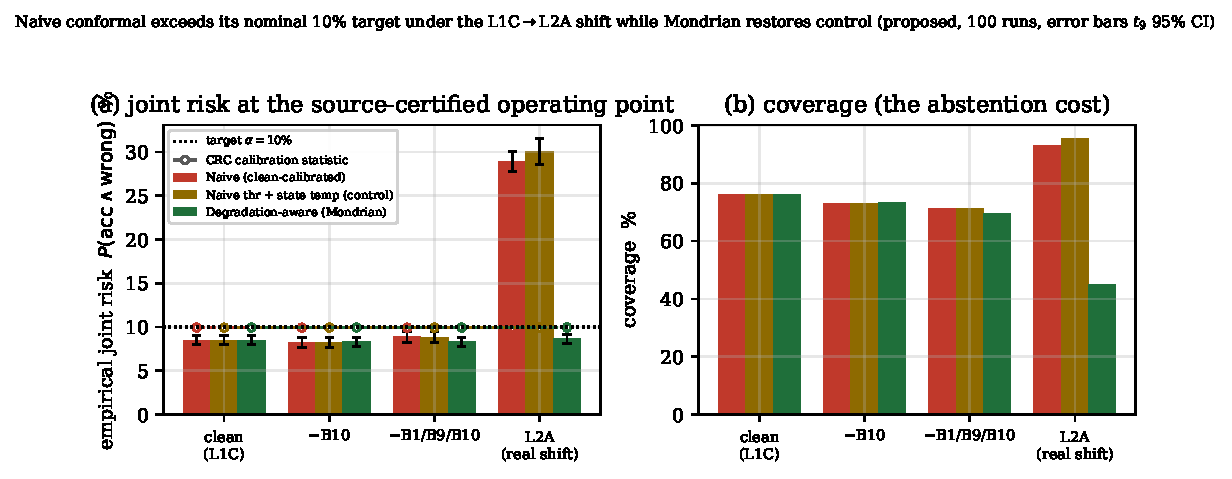
\includegraphics[width=\linewidth]{fig2_flagship_reliability.pdf}
\caption{Naive conformal exceeds its nominal $10\,\%$ target under the L1C$\to$L2A shift while Mondrian restores control (proposed model, 100 runs, two-way cluster-robust SE). (a) empirical joint risk at the certified operating point, per state, with error bars the small-cluster $t_9$ $95\,\%$ CI; (b) coverage, the abstention cost of the remedy. The dashed lines are the reused source-domain CRC calibration selection statistic (never re-validated on target outcomes), which stays $\leq \alpha$ throughout even as the naive L2A risk soars to $27.8\,\%$---the sense in which the failure is silent.}
\label{fig:flagship}
\end{figure}

\paragraph{The dominant mechanism is a stale input-normalization contract, and re-normalizing without labels reduces the risk to near the target.} Which part of the reflectance transformation is the certificate sensitive to---the per-pixel spectral distortion of the atmospheric physics, or the shift in each band's radiometric scale? The model normalizes every input with the per-band mean and variance of its \emph{source} (L1C) training data and reuses those statistics on L2A: a stale normalization contract that leaves the atmospherically-rescaled L2A input off the scale the certificate was calibrated on. We test the scale hypothesis directly by re-normalizing the L2A input with the \emph{target product state's} per-band statistics---estimated from an unlabelled target calibration sample, with no target labels and no change to the trained model, threshold or temperature---before the identical clean-calibrated certificate (ten model seeds $\times$ ten calibration splits on the flagship model). Product-aware re-normalization reduces the naive joint risk from $28.4 \pm 0.4\,\%$ (reproducing the flagship breach) to near the target: the operational, \emph{evaluation-disjoint} arm---statistics estimated on a target calibration split disjoint from the evaluation units, so no evaluation transduction---reaches $10.8 \pm 0.3\,\%$ at $74\,\%$ coverage (its interval $[10.1, 11.4]$ sitting just \emph{above} the $10\,\%$ target), and a pooled estimate agrees ($10.5 \pm 0.3\,\%$; paired difference $-0.2\,\%$ $[-0.6,+0.2]$, within noise). A richer label-free transport reaches the target level: a full per-band \emph{quantile} transport of the evaluation-disjoint arm---mapping each L2A calibration-band marginal onto the L1C-train marginal before the model's own standardization, still using no target labels and disjoint from the evaluation units---attains $9.6 \pm 0.2\,\%$ (interval $[9.0, 10.1]$) at $70\,\%$ coverage, its point estimate below the $10\,\%$ target and a significant improvement over first-two-moment standardization (paired reduction $+1.2\,\%$ $[+0.5, +1.9]$; part of it a modest $74\to70\,\%$ coverage reduction and part a genuinely cleaner accepted set, selective risk $14.5\to13.7\,\%$), with a robust two-moment transport intermediate ($10.2\,\%$). This is a large, \emph{label-free} reduction at clean-like coverage---a drop from ${\sim}28$ to ${\sim}10\,\%$, its strongest interval straddling the $10\,\%$ target rather than a formally re-derived $\leq\!10\,\%$ finite-sample guarantee---whose residual above clean ($8.5\,\%$) we do \emph{not} identify as physics---it is associated with non-affine or otherwise unmodelled product differences a global per-band rescaling cannot undo. We are explicit that three things differ: the \emph{empirical} risk is reduced to near target, but the re-normalization is estimated from deployment data (so it does not re-derive the source certificate's finite-sample guarantee) and it requires an unlabelled target calibration sample (here $69$ scene-components) rather than being fully data-free. A paired decomposition confirms the repair is specifically a \emph{product}-normalization effect, not generic test-time adaptation or a train-to-test scene-composition change: re-normalizing the L2A input with the \emph{paired L1C test-set} statistics---correcting scene composition but not the product---leaves the breach essentially unchanged (paired reduction $+0.0\,\%$ $[-0.1,+0.2]$), whereas swapping those for the L2A product's own statistics accounts for the \emph{entire} repair ($+17.9\,\%$ $[16.9,18.9]$), and re-normalizing the in-domain clean L1C to its \emph{own} test statistics slightly \emph{worsens} it ($+1.0\,\%$ $[0.7,1.2]$)---so the fix corrects a product-scale mismatch, not a free effect of test-batch re-normalization. Because these statistics are estimated from unlabelled deployment data, the re-normalization re-aligns the input so the source operating point \emph{transfers empirically}---restoring the empirical target joint-risk level on the deployment scenes rather than re-deriving a finite-sample guarantee. Two consequences reframe the mechanism and remedy that follow. First, the breach is \emph{dominated} by the calibration-to-deployment input-normalization mismatch---a stale contract between the certificate and the model's front end---rather than by the atmospheric physics as such. This does not contradict the failure of weighted conformal above; it explains it. Reweighting corrects the calibration distribution but cannot re-align an input that has moved almost entirely outside the calibration support, nor un-shift the off-scale scores it produces; product-aware re-normalization instead repairs the input \emph{upstream}, re-aligning the deployment product with the source---it collapses the clean-versus-L2A domain separability from AUROC $1.00$ to $0.56$---so the existing operating point transfers at a much lower empirical risk rather than being reweighted after the fact. Product-aware (test-time) input normalization is itself a long-known covariate-shift remedy \citep{adabn2016,schneider2020,nado2020,benz2021}, and the standard remote-sensing practice of a \emph{fixed} training normalization \citep{corley2024} is exactly the failing naive baseline here. Second, because a re-normalization estimated from an unlabelled target calibration sample reduces the risk to near the target at clean-like coverage, the per-stratum (Mondrian) recalibration we study is \emph{one} valid remedy but not the necessary, label-requiring one that the labelled arm alone would suggest: for the atmospheric shift the risk can be brought near target without any target labels or abstention (though the residual sits just above $10\,\%$ and the guarantee is not formally re-derived).

\paragraph{The label-free transport needs a representative target sample, not a fixed transform.}\label{par:renormgen} Because the quantile transport is estimated from an unlabelled target calibration sample, its operational value turns on how portable that estimate is; we probe this by re-estimating the mapping while varying only which and how many target components produce it, always deploying on a disjoint evaluation set (ten model seeds $\times$ ten calibration splits, two-way cluster-robust SE at $t_9$). Three readings result. It \emph{converges with sample size}: estimated on $8/16/24/40$ random calibration components the joint risk is $13.0/11.2/10.4/9.8\,\%$, approaching the full-calibration level ($9.6\,\%$; a paired excess of only $+0.3\,\%$ by forty components)---a few dozen components suffice but a handful do not. It is \emph{stable across random representative subsets}: two disjoint random halves reach $10.1$ and $9.9\,\%$, near target and near each other, so the near-target level is not an artefact of one particular calibration mixture. And it is \emph{not} a coverage artefact: coverage holds at ${\sim}70\,\%$ across every arm, so the risk differences are real, not bought by abstention. But it \emph{does} depend on the sample's surface composition: a mapping estimated on the bright half of the calibration components alone reaches only $12.5\,\%$, and on the dark half only $14.4\,\%$---both well above the ${\sim}10\,\%$ a random half of the \emph{same} size reaches---so the transport behaves as a batch-level adaptation that needs a moderately sized, surface-representative unlabelled target sample, not a single product-state transform portable from any subset. We do not test transfer across seasons, acquisition dates or processor baselines, which remains future work.

\paragraph{A second, algorithmically different atmospheric processor breaks it too.} If the breach were an artefact of Sen2Cor's particular radiometric conventions, a different processor should not reproduce it. We re-ran the flagship with ACOLITE---a dark-spectrum atmospheric correction at a fixed climatological aerosol optical thickness, algorithmically different from Sen2Cor---as an alternative L1C$\to$surface-reflectance product, on the $590$ test patches ACOLITE processed successfully ($181$ of the $184$ scene-components), evaluating every state on that same set with reflectance clipped to a physical range so that a small fraction of over-corrected bright pixels cannot drive the result (ACOLITE additionally omits the B9 water-vapour band, whose removal Table~\ref{tab:banddrop} shows is negligible). The naive certificate breaks to a statistically equivalent degree under the two processors: ACOLITE-surface naive joint risk is $29.6 \pm 0.6\,\%$ (its $t_9$ interval $[28.2, 31.0]$ excluding the target), against $29.3 \pm 0.8\,\%$ for Sen2Cor-L2A on the same patches ($29.60$ and $29.34\,\%$)---their paired per-run difference is $+0.26\,\%$ with a bootstrap interval $[-1.02, +1.42]$ lying within a $\pm 2\,\%$ equivalence margin (a two-one-sided test, which passes), so the two independently-implemented corrections break the certificate equivalently rather than merely landing close in point estimate---and $9.3\,\%$ on clean L1C, with Mondrian restoring both ($9.1$ and $8.7\,\%$). That two algorithmically different processors break the source-calibrated certificate near-identically shows the failure is not an artefact of one processor's radiometric conventions; because both implement a broadly similar top-of-atmosphere-to-surface transformation, this points to the L1C$\to$surface-reflectance shift rather than to Sen2Cor specifically, though it does not on its own isolate the atmospheric physics from conventions the two processors may share. Two controls (Appendix~\ref{app:repro}) confirm the comparison is neither an artefact of \emph{which} scenes ACOLITE could process nor of the reflectance clip: the ACOLITE-retained cohort is not strongly imbalanced from the ACOLITE-failed one on the observed covariates (cloud cover $p=0.38$, latitude $p=0.38$, effect sizes negligible-to-small), though because ACOLITE cannot process the failed scenes their ACOLITE risk is unidentified---we report the ACOLITE result conditional on successful processing---and the ACOLITE breach stays within $28.6$--$31.6\,\%$ across no clip, the $[-0.1,1.6]$ clip and a tight $[0,1]$ clip---if anything the clip \emph{lowers} it.

\paragraph{The breach replicates on a within-dataset held-out scene set.} A single test split cannot show the phenomenon is not specific to those $195$ scenes. We therefore repeat the flagship protocol on the official CloudSEN12 \emph{validation} split---$535$ high-quality-labelled patches from $107$ annotation ROIs ($104$ scene-connected components). This split is a random draw from the non-test scenes rather than a spatially blocked hold-out, so while it is disjoint from the test scenes by construction it can share Sentinel-2 products with train; we therefore audited it, found two products also present in train, and dropped their pixels ($0.4\,\%$ of the set) so the replication is genuinely calibration-disjoint from training. We use this split only as an independent replication set, never for model selection or tuning. Training the identical model on the same train split and calibrating and evaluating the CRC on the audited held-out scenes, the failure reproduces: the naive joint risk rises from $8.1\,\%$ on clean L1C to $28.0 \pm 0.7\,\%$ under the L1C$\to$L2A shift (its $t_9$ interval $[26.3, 29.6]$ excluding the target), the confidence ranking degrades in step (AURC $6.2 \to 21.6$, a $3.5\times$ rise), and Mondrian restores the target ($7.8\,\%$) at the same coverage cost ($93 \to 42\,\%$). The per-class collapse recurs as well: mean IoU falls $54.4 \to 30.0$ and the two minority cloud classes collapse almost completely (thin cloud IoU $34.4 \to 1.6$, shadow $35.0 \to 2.9$), their accepted-pixel selective risk reaching $99.8\,\%$, so the confidently-wrong mass concentrates in the same minority classes as on the test split (Table~\ref{tab:classwise}). The magnitude on a within-dataset held-out set of scenes is within a point of the test-split headline, so the atmospheric-certificate failure is a property of the task and shift, not of the particular scenes calibrated on (a within-dataset held-out replication, not a fully independent dataset).

\paragraph{Pixel accuracy hides a per-class collapse.} The aggregate accuracy drop understates the operational damage and conceals \emph{which} pixels fail. Decomposing the flagship by class (Table~\ref{tab:classwise}; the full $10\times10$ design), the shift crashes the mean IoU from $53.8$ to $29.9$ and macro-F1 from $67.7$ to $38.2$: the two minority cloud classes---thin cloud and cloud shadow, operationally the hardest and most label-ambiguous \citep{aybar2022cloudsen12}---collapse almost completely (IoU $30.5\to0.4$ and $37.4\to2.5$). That is exactly where the confidently-wrong mass concentrates: at the clean-calibrated operating point, the accepted-pixel error rate (selective risk) on L2A reaches $99.9\,\%$ for thin cloud and $98.8\,\%$ for cloud shadow, while the dominant clear class retains a low empirical selective risk ($1.1\,\%$). The confidently-wrong mass is thus not diffuse---it is driven by minority-class failures that overall pixel accuracy masks (the pixel-support-weighted sum of the class-conditional joint risks, $\sum_k w_k R_k$ with $w_k$ the class-$k$ pixel fraction, is $28.2\,\%$, recovering the pixel-pooled joint---which matches the $27.8\,\%$ component-equal headline to within the component-versus-pixel weighting difference), which is why we read the accuracy drop as an \emph{under}-statement of the operational damage. Operationally the confidently-wrong mass is thin cloud and shadow admitted as clear, so any downstream product that trusts the naive certificate---a cloud-screened composite, a surface-reflectance time series---would ingest cloud- and shadow-contaminated pixels precisely where the certificate reports itself in control.

\begin{table}[t]
\centering
\caption{Per-class decomposition of the flagship over the full $10\times10$ design (proposed model, ten model seeds $\times$ ten calibration splits; IoU and the CRC risks are mean $\pm$ two-way cluster-robust standard error, coverage is the mean). Pixel accuracy hides the shift's effect: under L2A the minority cloud classes collapse in IoU and the confidently-wrong mass concentrates in them (their accepted-pixel selective risk saturates near $100\,\%$; the subscripts give the min--max over the 100 cells, so it is a genuine saturation, not a single-split artefact), while the dominant clear class retains low selective risk. The per-class quantities are empirical class-conditional risks---conditioned on the true-class pixels---not class-conditional conformal guarantees; the CRC operating-point risks are at the clean-calibrated threshold. Class pixel supports on L2A are clear $51\,\%$, thick cloud $30\,\%$, thin cloud $10\,\%$, cloud shadow $10\,\%$, so the two collapsing minority classes are only ${\sim}19\,\%$ of pixels yet drive the joint risk. All values in \%.}
\label{tab:classwise}
\begin{tabular}{llcccc}
\toprule
state & class & IoU & selective risk & joint risk & coverage \\
\midrule
clean & clear        & $76.4\pm0.2$ & $2.6\pm0.2$ & $2.23\pm0.15$ & 84.6 \\
      & thick cloud  & $71.0\pm0.3$ & $9.2\pm0.4$ & $7.04\pm0.31$ & 76.3 \\
      & thin cloud   & $30.5\pm0.8$ & $57.8\pm1.8$ & $26.06\pm1.00$ & 45.2 \\
      & cloud shadow & $37.4\pm0.8$ & $48.7\pm1.4$ & $27.99\pm0.98$ & 57.4 \\
\midrule
L2A   & clear        & $61.6\pm0.6$ & $1.1\pm0.5$ & $1.04\pm0.46$ & 95.9 \\
      & thick cloud  & $55.3\pm1.2$ & $40.3\pm1.7$ & $35.15\pm1.40$ & 87.2 \\
      & thin cloud   & $\mathbf{0.4\pm0.2}$ & $\mathbf{99.9}_{[99,100]}$ & $90.36\pm0.73$ & 90.4 \\
      & cloud shadow & $\mathbf{2.5\pm0.7}$ & $\mathbf{98.8}_{[92,100]}$ & $89.64\pm1.59$ & 90.7 \\
\bottomrule
\end{tabular}
\end{table}

\paragraph{The breach is not an artefact of the weighting.} The certified triple is component-equal-weighted (Section~\ref{sec:unit}) whereas the segmentation accuracy is pixel-level, so we re-evaluated every flagship quantity at the same operating point under the pixel-pooled (sample-weighted) alternative, on an independent $100$-run draw. The two weightings agree to within noise: the L2A naive joint risk is $28.3\,\%$ component-equal versus $28.3\,\%$ pixel-pooled (coverage $92.7$ versus $92.7\,\%$; selective risk $30.0$ versus $30.0\,\%$), and the component-equal accuracy equals the pixel accuracy ($67.9\,\%$). The scene-connected components are close enough in size that the choice of weighting does not move the headline, and the component-equal joint of $28.3 \pm 0.8\,\%$ reproduces the flagship's $27.8\,\%$ on this fresh set of seeds.

\subsection{Two pure deployment shifts: a suggestive surface excess, no clear geographic breach}
\label{sec:deployment}
To test whether the failure is specific to the atmospheric shift we construct two further shifts of a different \emph{type} on the same task, holding the input product fixed (clean L1C) so that the shift is \emph{where the model is deployed}, not \emph{what bands it sees}. In each, the naive arm calibrates on held-out source units and is evaluated on unseen target units; the Mondrian arm recalibrates on the target (Fig.~\ref{fig:gaps}). The surface strata (dark: vegetation, cropland, water; bright: built-up, bare soil, snow/ice) and the hemispheric split (by scene-centroid latitude) follow fixed rules; the exact assignment and the per-stratum scene, season and class-proportion breakdown are given in the released code.

\emph{Surface domain gap.} Training and naive-calibrating only on dark surfaces (vegetation, cropland, water) and deploying on the bright surfaces (built-up, bare soil, snow/ice) the model has never seen---the operational cloud-confusion case---raises the naive joint risk to a suggestive $11.34 \pm 0.45\,\%$---its small-cluster $t_9$ interval $[10.3, 12.4]$ excludes $10\,\%$, but the fuller scene-component bootstrap over the $33$ bright units is inconclusive ($[9.0, 14.4]$, Section~\ref{sec:method}); Mondrian restores it to $2.39 \pm 0.21\,\%$. The plain-MLP-with-band-group-dropout baseline (b2) mirrors this ($11.9 \to 2.5\,\%$), so the effect is not architecture-specific.

\emph{Geographic domain gap.} Training and calibrating on the Northern hemisphere and deploying on the unseen Southern hemisphere, under the identical 100-run design, shows no clear evidence of exceeding the target: the proposed model's naive joint risk on Southern units is $9.71 \pm 0.26\,\%$ (its $t_9$ interval $[9.1, 10.3]$ and a scene-component bootstrap $[9.1, 12.4]$ both including the $10\,\%$ target), and the plain-MLP baseline likewise straddles it ($10.12 \pm 0.23\,\%$, $t_9$ interval $[9.6, 10.6]$). Neither is the clear violation the surface gap produced. Accuracy also transfers well ($79\,\%$ on Southern units), consistent with Northern and Southern mid-latitudes sharing surface and cloud regimes. Mondrian still lowers the risk further (proposed $5.7\,\%$), but from an already-controlled starting point.

The surface and geographic axes are both pure deployment shifts on a fixed input, so the contrast is between two operational shifts of different kinds; we do not claim they differ only along a single measured gap dimension---the surface and hemisphere splits also differ in class prevalence, season and biome. The structural surface gap (dark training surfaces to spectrally very different bright ones) suggestively exceeds the naive certificate's target; the milder geographic gap (regions that share surface and cloud regimes) shows no clear breach. A direct paired bootstrap of the surface-minus-geographic difference confirms this is more than a one-significant-one-not artefact: the difference is $+1.62\,\%$, its $95\,\%$ interval $[+0.95, +2.35]$ excluding zero, so the surface axis breaches significantly more than the geographic one---though both sit close to the target in absolute terms. This is an illustrative contrast between two deployment shifts: the surface gap suggestively exceeds target (inconclusive under full resampling, but significantly above the geographic axis), while the milder geographic gap gives no clear evidence of a breach. We read it as suggestive of a \emph{conditional} failure---one that appears under the bright-surface split but not the hemisphere split---rather than as a general diagnosis or a claim that severity tracks a measured gap size. The atmospheric shift breaks harder still ($27.8\,\%$) but also changes the input representation, so we read it as a stronger, different-mechanism confirmation rather than another point on the same deployment-gap scale.

On the surface axis the Mondrian arm recalibrates on a median of only ${\sim}12$ scene-component units (versus ${\sim}91$ for the naive arm and ${\sim}69$ for the flagship). At $\alpha = 10\,\%$ this is near the conformal feasibility floor, so the restored $2.4\,\%$ at $41\,\%$ coverage (full triple in Table~\ref{tab:deploytriple}) reflects heavy, conservative over-abstention on a small target stratum rather than a tight guarantee at target---we report it as restoring \emph{control at a large coverage cost}.

\begin{figure}[t]
\centering
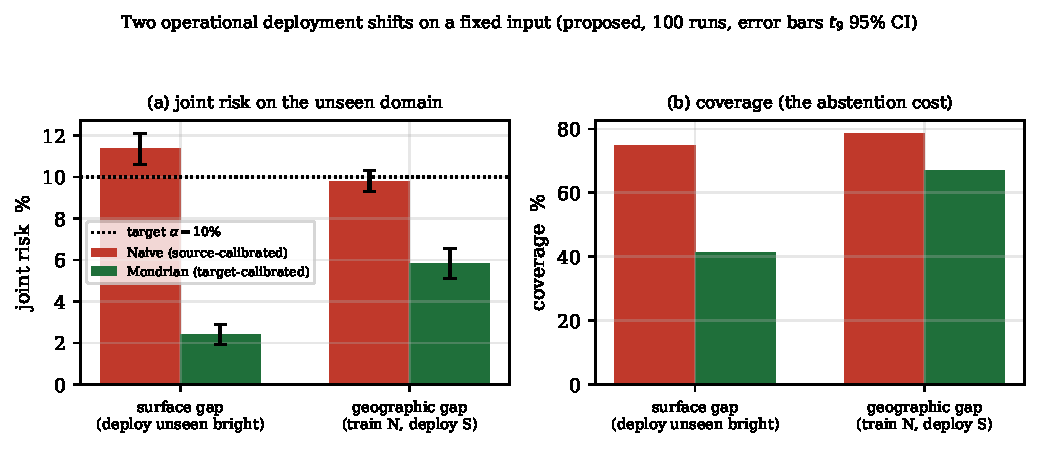
\includegraphics[width=0.6\linewidth]{fig3_domain_gaps.pdf}
\caption{Naive versus Mondrian joint risk on the unseen target domain, for the surface and geographic deployment shifts (proposed model). The structural surface gap produces a suggestive excess above the $10\,\%$ target (inconclusive under full calibration resampling); the milder geographic gap shows no clear breach.}
\label{fig:gaps}
\end{figure}

\begin{table}[t]
\centering
\caption{Full operating-point triple for the two deployment shifts (proposed model, 100 runs; joint-risk SE two-way cluster-robust). Reporting selective risk and coverage alongside the joint risk shows that the surface Mondrian's low joint risk ($2.4\,\%$) is bought with heavy abstention (coverage $41\,\%$) rather than a genuinely reliable accepted set, and that the geographic naive arm is already near target. Accuracy is on the target domain. All values in \%.}
\label{tab:deploytriple}
\begin{tabular}{llcccc}
\toprule
shift & arm & joint risk & selective & coverage & accuracy \\
\midrule
surface    & naive    & $11.34\pm0.45$ & $15.3\pm0.6$ & $74.3\pm1.0$ & $75.1\pm0.9$ \\
           & Mondrian & $2.39\pm0.25$  & $5.8\pm0.4$  & $39.9\pm2.3$ & $75.1\pm0.9$ \\
\midrule
geographic & naive    & $9.71\pm0.26$  & $12.4\pm0.4$ & $78.6\pm0.7$ & $79.2\pm0.6$ \\
           & Mondrian & $5.72\pm0.36$  & $8.5\pm0.5$  & $66.9\pm0.7$ & $79.2\pm0.6$ \\
\bottomrule
\end{tabular}
\end{table}

\subsection{A model-specific comparison}
\label{sec:modelclass}
We run a frozen channel-adaptive foundation model \citep[DOFA,][]{xiong2024dofa} through the \emph{identical} flagship protocol---the same CRC joint-risk estimand, the scene-connected-component unit, the $10 \times 10$ crossed design, and the two-way cluster-robust SE---so the CRC \emph{protocol} is identical across the two models, though their capacity, pretraining and spatial context are not. DOFA is \emph{far more} reliable than the small per-pixel model under the L1C$\to$L2A shift: naive joint risk $9.95 \pm 0.21\,\%$ versus $27.8\,\%$ for the small model. Its L2A joint risk sits right at the $10\,\%$ target (its small-cluster $t_9$ interval $[9.4, 10.5]$ including it), so a clear residual breach cannot be established; Mondrian lowers it to $8.79 \pm 0.19\,\%$, and the abstention cost is far gentler than the flagship's (coverage $80.0 \to 76.4\,\%$, versus $93 \to 48\,\%$ for the small model). DOFA is not immune, however: under a spectral-band-drop shift (removing its two SWIR bands) its naive joint risk rises to $11.77 \pm 0.42\,\%$, its $t_9$ interval $[10.9, 12.6]$ excluding the target---a breach now certified over the full $10 \times 10$ design---and Mondrian brings it to $8.63 \pm 0.36\,\%$. The reliability crisis is thus \emph{model-specific} in this two-model comparison: a channel-adaptive foundation model largely escapes it under the atmospheric shift but shows a modest, certified breach under a band-drop shift, and we do not claim a universal failure. We cannot fully decompose \emph{which} of DOFA's differences produces the greater reliability, but first principles narrow them. Channel-adaptivity is not the differentiator: our small model is itself a wavelength-conditioned band-as-modality encoder. Two differences are mechanistically pointed. First, DOFA's fixed nine-band input omits the water-vapour band B9, whose reflectance shifts most of any band under the L1C$\to$L2A correction (by ${\sim}{+}0.2$--$0.3$ here), while the flagship's thirteen-band input uses it: a model that never sees the most atmospherically-volatile band is by construction less exposed to the shift, so a fully fair model-class comparison would additionally control the band set. We test this directly: a plain per-pixel MLP---no spatial context, no pretraining---trained and calibrated identically on three band sets breaks the naive certificate to $48.4 \pm 0.2\,\%$ on all thirteen L1C bands, but to only $29.2 \pm 0.5\,\%$ once B9 alone is removed and $24.1 \pm 0.3\,\%$ on DOFA's exact nine bands. Dropping the single most volatile band thus accounts for most of the band-set effect, and the band set as a whole roughly halves the breach---a concrete, quantified contributor to DOFA's greater reliability that a fair comparison must control. The same three-band-set ablation on the band-as-modality flagship itself reproduces this pattern---$28.3 \pm 0.4\,\%$ on all thirteen bands, $22.6 \pm 0.7\,\%$ without B9, $21.1 \pm 0.8\,\%$ on DOFA's nine (this variant additionally re-partitions the flagship's spectral groups, so it is a coarser test than the fixed-architecture MLP)---so the flagship's headline breach is not an artefact of the single most atmospherically-volatile band. It does not close the gap on its own, though: even the nine-band per-pixel MLP ($24.1\,\%$) sits far above DOFA's $9.9\,\%$, leaving the residual to DOFA's spatial context and pretraining. Second, DOFA's spatial context can resolve the per-pixel-ambiguous thin-cloud and shadow pixels that drive the breach from their spatial neighbourhood, which a per-pixel model cannot; its cross-modal pretraining plausibly adds shift-stable features on top. These causes are entangled and we claim no decomposition: the escape is multi-causal, with the band set a concrete contributor a fair comparison must control, so we read the DOFA result as establishing that a different model \emph{class} largely escapes the failure, not the single mechanism behind it. (This is a foundation-model \emph{feature} baseline---a frozen encoder with a light trainable head, not the official DOFA segmentation recipe.) DOFA's Sentinel-2 pretraining imagery derives from SatlasPretrain \citep{bastani2023}, which samples the global 2016--2022 archive; because CloudSEN12's 2018--2020 acquisitions fall inside that envelope, incidental scene overlap cannot be fully excluded. But DOFA is pretrained self-supervised on raw reflectance with no cloud labels and is used here only as a frozen extractor (no fine-tuning), and SatlasPretrain preferentially retains low-cloud scenes whereas CloudSEN12 targets cloudy ones, so any overlap is non-systematic and introduces no cloud-mask label information into our result, though we cannot exclude that pretraining exposure shapes its representation.

\paragraph{Spatial context, isolated in a matched convolutional family, modestly attenuates the breach without removing it, and the label-free fix generalizes.} DOFA differs from the per-pixel model in band set, spatial context and pretraining at once, so no two-model comparison isolates spatial context cleanly. We isolate the \emph{receptive field}---the structural correlate of spatial context---inside one matched convolutional family: on DOFA's exact nine bands, trained from scratch, we build a depth-, width-, optimizer-, epoch-, batch- and training-sample-matched convolutional stack in which the kernel size is the \emph{only} structural knob (a $1\times1$ stack is a per-pixel model applied convolutionally; $3\times3/5\times5/7\times7$ grow the receptive field to $9/17/25$ pixels), and pass every arm through the identical certificate (five model seeds $\times$ ten calibration splits; all arms trained full-patch, so the training regime is held fixed and cannot confound the contrast). Along the raw kernel sweep the stale-normalization breach attenuates monotonically---$20.4 \to 19.8 \to 17.9 \to 17.4\,\%$ from $1\times1$ to $7\times7$ (paired $1\times1$ minus $7\times7$ $+3.0\,\%$ $[+0.03,+6.0]$)---but kernel size and parameter count co-grow along it, so to isolate the receptive field we add \emph{capacity-matched} $1\times1$ controls: a width-inflated per-pixel arm carrying the same parameter count as each $k\times k$ arm (${\sim}30$k, ${\sim}85$k, ${\sim}165$k parameters), so each matched pair holds the parameter budget fixed and differs only in whether that budget buys a receptive field (the $k\times k$ arm) or extra width (the wide $1\times1$, still zero-context). At matched capacity the receptive field itself attenuates the breach at the two larger fields---$+2.11\,\%$ $[+1.79,+2.42]$ at $17$px ($1\times1$-wide minus $5\times5$) and $+3.42\,\%$ $[+1.34,+5.50]$ at $25$px ($1\times1$-wide minus $7\times7$), both two-way intervals excluding zero---but is \emph{not} resolved at the smallest $9$px field ($+0.74\,\%$ $[-1.75,+3.22]$, including zero). Widening the network at a fixed $1\times1$ field moves the breach at none of the three matched capacities (capacity-only contrasts $-0.16$, $+0.44$, $-0.41\,\%$, every two-way interval including zero); nor is the attenuation an under-fitting artefact of the wide controls, which fit clean at least as well as their $k\times k$ partners (all seven arms reach $7.9$--$8.9\,\%$ clean joint risk on L1C), so the zero-context arms' larger breach is shift-specific. Within this family it is thus spatial context (receptive field), not capacity, that attenuates the breach---resolved only at receptive fields of $17$px and above, modest (${\sim}2$--$3$ points) and scoped to the family, not a fixed point count transferable across architectures. A one-harness per-pixel-MLP-versus-U-Net comparison on the same nine bands corroborates the direction with a larger gap ($23.6 \pm 0.6\,\%$ versus $14.4 \pm 0.9\,\%$), but that gap co-varies architecture, parameter count, convolutional inductive bias and training regime, so we read it as a same-direction confirmation, not a clean causal estimate---either way a representative spatial model breaches the certificate too, so the failure is \emph{not} a per-pixel artefact. The DOFA foundation model is separately far more reliable ($9.9\,\%$), but as it changes architecture, capacity, band representation, pretraining corpus and output head at once, its advantage cannot be attributed to pretraining alone: that pretraining adds shift-stable features on top of spatial context is a \emph{hypothesis} consistent with the ordering ($23.6 \to 14.4 \to 9.9\,\%$), not a factorial decomposition. We therefore report the reliability crisis as \emph{model-specific across the tested models}---most severe for the per-pixel spectral model and, within a matched family, modestly attenuated by a larger receptive field---rather than as a decomposable per-mechanism gradient. The label-free remedy generalizes with the failure: product-aware re-normalization (pooled target statistics) reduces \emph{every} arm to near the target at clean-like coverage (per-pixel MLP $23.6 \to 8.8\,\%$ at $69\,\%$, U-Net $14.4 \to 8.9\,\%$ at $78\,\%$, and each matched-kernel arm to $9$--$11\,\%$), so the input-normalization contract diagnosed on the flagship is not specific to any one architecture.

\begin{table}[t]
\centering
\small
\caption{The naive certificate's confidently-wrong (joint) risk and its per-stratum (Mondrian) restoration across every condition tested, against the $10\,\%$ target (mean $\pm$ two-way cluster-robust SE, \%). The atmospheric breach reproduces under a second, algorithmically different processor, on held-out validation scenes, and---separately---across target risks $5$--$20\,\%$, and covariate-shift weighted conformal does not restore a useful operating point (source-only heuristics reach $32.2$--$32.6\,\%$; a formal component-level weighted CRC holds the joint risk valid only by abstaining to $7\,\%$ coverage), whereas a label-free product-aware re-normalization brings the empirical risk to $10.8\,\%$ at $74\,\%$ coverage. Among pure deployment shifts it is conditional; under the identical protocol a channel-adaptive foundation model is far more reliable to the atmospheric shift, and a matched-kernel convolutional isolation (capacity controlled) attributes a modest part of that gap to spatial context (receptive field). Breach $=$ the small-cluster $t$ interval excludes the target.}
\label{tab:summary}
\begin{tabular}{lccl}
\toprule
Condition & Naive & Mondrian & Verdict \\
\midrule
\multicolumn{4}{@{}l}{\emph{Atmospheric shift L1C$\to$L2A, small per-pixel model}} \\
\quad Sen2Cor, test (flagship)    & $27.8 \pm 0.8$ & $8.6$ & breach \\
\quad ACOLITE, test               & $29.6 \pm 0.6$ & $9.1$ & breach \\
\quad Sen2Cor, validation scenes  & $28.0 \pm 0.7$ & $7.8$ & breach \\
\midrule
\multicolumn{4}{@{}l}{\emph{Deployment shift (input fixed), small per-pixel model}} \\
\quad Surface, dark$\to$bright    & $11.3 \pm 0.5$ & $2.4$ & suggestive$^{\dagger}$ \\
\quad Geographic, North$\to$South & $9.7 \pm 0.3$  & $5.7$ & no clear breach \\
\midrule
\multicolumn{4}{@{}l}{\emph{Foundation model (DOFA), identical protocol}} \\
\quad Atmospheric L1C$\to$L2A     & $9.9 \pm 0.2$  & $8.8$ & no clear breach \\
\quad Spectral band drop (SWIR)   & $11.7 \pm 0.4$ & $8.6$ & breach \\
\bottomrule
\end{tabular}

\vspace{2pt}
{\footnotesize $^{\dagger}$ suggestive excess, inferentially inconclusive: significant under the two-way SE ($[10.3,12.4]$) but the full nested calibration-resampling bootstrap ($[9.5,14.2]$) includes the target; it is, however, significantly above the geographic axis (difference $+1.62\,\%$ $[+0.95,+2.35]$).}
\end{table}

\section{Discussion and limitations}
\label{sec:disc}
We lead with the limitations, because several bound the claims directly.

\paragraph{Coverage and selective risk are part of the result, not a footnote.} The certified quantity is a joint mass, which any method drives to zero by abstaining. Mondrian's restoration is therefore genuine but partial: on the flagship it accepts $48\,\%$ of pixels where naive accepts $93\,\%$, and even among those it accepts the error rate is $18.2\,\%$, not $\leq\!10\,\%$---what is controlled is the \emph{joint} confidently-wrong mass, not the accepted-pixel error rate. The operational reading is that per-stratum recalibration converts a silent, uncontrolled joint error mass into an \emph{explicit} accuracy--coverage trade the operator can see and choose. We report every risk with both its coverage and its selective error precisely so this trade is never hidden.

\paragraph{Across two deployment shifts, a breach appears under one but not the other.} The surface and geographic axes are both pure deployment shifts on a fixed input, so the comparison is between two deployment shifts of different kinds: the structural surface gap produces a suggestive excess above target ($11.3\,\%$, its two-way SE interval excluding the target but the full nested calibration-resampling bootstrap including it), while the milder geographic gap shows no clear evidence of a breach ($9.7\,\%$, its $t_9$ interval including the target). A breach appears under this structural domain gap between calibration and deployment but not under this milder geographic split---so within this pair it is the \emph{kind} of shift, not mere geographic distance, that coincides with the breach; but with only two hand-chosen splits, which also co-vary class prevalence, season, biome and calibration size, and with no independently-measured domain-gap metric, we do not read this as a general law that whether a breach occurs is determined by shift kind. The atmospheric shift breaks harder ($27.8\,\%$) but also changes the input representation, so we read it as a stronger, different-mechanism confirmation. We do not claim a smooth monotone ``severity $= f(\text{gap size})$'' law---an independently-measured gap metric across more shift types would be needed---and we read the surface-above-target / geography-shows-no-clear-breach pair as an illustrative contrast of two deployment shifts, not a general diagnosis. The crisis is also model-specific---a larger pretrained foundation model is far more reliable under the atmospheric shift, so the severity does depend on the model, with the small per-pixel model suffering it most. Within a matched convolutional family we can isolate one structural correlate cleanly: at matched capacity a larger receptive field (resolved at $17$px and above) modestly attenuates the breach (${\sim}2$--$3$ points, capacity-matched contrasts excluding zero), so within the family, allocating capacity to a larger receptive field rather than $1\times1$ width is \emph{associated} with the attenuation---though this within-family contrast does not separate spatial context from the convolutional spatial regularization a larger kernel also introduces (they co-vary in FLOPs and optimisation geometry), rests on five model seeds ($t$ at four degrees of freedom), and is not resolved at the smallest $9$px field. The foundation model's advantage separately co-varies capacity, pretraining, band representation and output head, so we do not attribute it to any single one of those differences.

\paragraph{Scope of the evidence.} The magnitude is measured on one benchmark (CloudSEN12); its test metadata records eight distinct Sen2Cor product-baseline versions, a mild internal heterogeneity we do not control for. We have, however, stressed the finding along every axis this benchmark affords: two algorithmically different atmospheric processors (Sen2Cor and ACOLITE) break it to a statistically equivalent degree, it replicates on the official held-out validation scenes (audited for shared train products, $28.0\,\%$ versus the $27.8\,\%$ headline), it survives target risks from $5$ to $20\,\%$ and both deployment-shift axes, and it is model-specific across the tested models (a channel-adaptive foundation model largely escapes it). What remains outside this benchmark's reach is a \emph{fully independent} cloud dataset with its own labelling protocol and geography; because no public Sentinel-2 cloud-segmentation dataset ships paired L1C/L2A at CloudSEN12's expert label quality, establishing the magnitude on a second dataset requires re-processing raw products through an atmospheric-correction pipeline and is the most direct further strengthening.

\paragraph{The mechanism is borrowed; the comparison is not compute-matched.} Our band-as-modality architecture is a substrate of cited components, and the proposed-vs-MLP comparison is not matched on training compute, optimiser steps, or data exposure. The paper's claim is the \emph{within-method} naive-vs-Mondrian gap, invariant to that confound because both arms share the trained model; the plain-MLP baseline reproducing the surface-axis result ($11.9 \to 2.5\,\%$) shows the finding does not depend on it.

\paragraph{Statistical caveats.} The exchangeable unit is the scene-connected component and the standard error is two-way cluster-robust; these were found by adversarial review and change the confidence intervals, not the direction of the result. The scene-connected component is a reasonable operational approximation to exchangeability, not a proof of it: residual dependencies remain---the same annotation region on different dates, adjacent regions, a shared acquisition or atmospheric system, and the reuse of a component across the Monte-Carlo splits. The seed-cluster bootstrap, seed-only aggregation and a scene-component bootstrap of the evaluation composition (Section~\ref{sec:method}) leave the flagship breach intact; for the borderline surface breach we additionally ran a nested scene-component bootstrap that, on each of $600$ resamples, re-draws a bright/dark scene cohort shared across all ten model seeds, re-splits temperature and calibration, re-fits the temperature and re-selects the CRC threshold, and re-computes the \emph{seed-averaged} joint risk---the estimator the headline reports---so it propagates calibration-composition uncertainty in the reported estimand itself (every resampled cell CRC-feasible). Its $95\,\%$ interval is $[9.5, 14.2]$ (mean $11.7\,\%$): the point estimate remains above target but the interval includes $10\,\%$, so under full calibration resampling the surface breach is inferentially inconclusive---consistent with the evaluation-only bootstrap ($[9.3, 13.6]$) and reinforcing our reading of it as suggestive rather than settled. With only 10 clusters on each factor our cluster-robust intervals are themselves small-cluster approximations; we therefore read the borderline geographic axis as suggestive rather than settled. \citet{barber2023}'s coverage-gap bound is worst-case and does not predict our exact numbers. The estimand is the mean risk on a fixed per-patch pixel sample (one sampling seed across runs), so our standard error reflects the calibration-split and model-seed variation, not pixel-sampling variability---a residual source we bound by using several hundred pixels per patch but do not fully propagate.

\paragraph{Alternative explanations we cannot fully exclude.} We trace the atmospheric breach to a stale normalization contract, but several co-factors remain only partially controlled, and the residual above clean is \emph{not} identified as atmospheric physics. The residual after re-normalization (${\sim}1$--$2$ points) we attribute to non-affine or otherwise unmodelled product differences an affine per-band rescaling cannot undo---candidates include quantile-map estimation error, cross-band (joint) dependence that a per-band marginal transport does not preserve, a residual class-conditional spectral mismatch, and processor-specific resampling or invalid-value handling---rather than to any identified physical mechanism. A class-prior shift between the L1C and L2A pixel populations is \emph{not} a candidate: the paired flagship shares identical pixels and labels across the two product states, so $P(Y)$ is fixed by construction and only a train-to-test prior difference is possible. The minority-class collapse co-occurs with the greater label ambiguity of thin cloud and shadow \citep{aybar2022cloudsen12}; we read this as an association, not as evidence that label ambiguity \emph{causes} the collapse. Our uncertainty score is the maximum softmax probability, a deliberately simple and known-fragile confidence; a sharper score could narrow or widen the gap. The label-free re-normalization depends on the composition of the unlabelled target calibration sample and on its stationarity---a mapping estimated on one batch of scenes may drift on future dates or other regions---within the test scenes it already needs a moderately sized, surface-representative calibration sample (Section~\ref{sec:flagship}), and cross-date/cross-region transfer is untested---and the estimated-weight analysis rests on a domain classifier whose likelihood ratio may be miscalibrated near separability. That near-separability is itself an \emph{empirical} statement---a domain classifier reaching AUROC${\approx}1$, i.e.\ poor finite-sample overlap---not a proof that the L1C and L2A supports are mathematically disjoint. Same-region multi-date and adjacent-scene dependence, the fixed pixel-sampling draw, and DOFA's incidental self-supervised exposure to overlapping scenes are further residual couplings our splits bound but do not eliminate. The U-Net-versus-MLP gap co-varies capacity and optimisation, which is why we lead the spatial claim with the matched-kernel family instead. And our AURC/AUGRC rises conflate genuine ranking degradation with the higher base error rate under shift; the base-rate-invariant failure-detection AUROC, which degrades in step, is the more direct ranking measure. None of these overturns the naive-versus-recalibrated gap---within-model, sharing the trained network---but each qualifies the mechanism's decomposition rather than the headline failure.

\paragraph{Implications.} For operational Earth observation the practical message is narrow and actionable: a model must not be assumed \emph{reliable} under a shift on the strength of its \emph{aggregate} accuracy---which can hold up while hiding a per-class collapse and a silent certificate failure---and a conformal or selective-prediction operating point calibrated before deployment should be treated as valid only within the calibration regime. The failure we characterise is the \emph{silent} reuse of one certificate when the shift is not flagged as a distinct operational state: an unlabelled processing-baseline change, a gradual sensor drift, or a pipeline that freezes its input normalization and threshold at training time. The remedies form a hierarchy of increasing cost. When the shift is a known input-processing change that the scene metadata already records---the L1C-versus-L2A product level is the clearest case---the first response needs \emph{no labels}: re-normalize with the target product state's statistics, estimated from an unlabelled target calibration sample, before inference, which on the atmospheric shift reduces the risk to near the target ($10.8\,\%$, just above $10\,\%$) at clean-like coverage (Section~\ref{sec:flagship}). The operational contract is simply that the input normalization travel with the product rather than be frozen at training time; a metadata gate on product level triggers it automatically. Where a residual remains, or the operational state is discrete but not a mere normalization change (our surface gap), per-stratum (Mondrian) recalibration is the next safeguard, at a cost the operator can see and choose---target-state labels to recalibrate on, and abstention. Where the shift is continuous or unknown, the online adaptive-conformal machinery we did not invoke here (beyond the source-only weighted thresholds we did test) is the natural next tool, and quantifying its cost under the same operational shifts is future work.

\paragraph{Companion analyses.} Two further analyses inform but do not carry the main result---a training-ingredient decomposition showing that \emph{synthetic} band-removal robustness overstates \emph{physically-grounded} (6S) band-loss robustness, and an exploratory EMIT external anchor that aligns only weakly with our per-band anomaly. We relegate their detail to Appendix~\ref{app:companion} to keep the main line on the load-bearing CloudSEN12 conformal experiments.

\section{Conclusion}
Robustness certification is not reliability certification. On real Sentinel-2 cloud segmentation, under the operational L1C$\to$L2A atmospheric-correction shift a model's \emph{aggregate} accuracy understates the operational damage (a 12-point drop that masks a per-class collapse) while a naive conformal certificate comes to admit more than three times the confidently-wrong risk it reports---silently, because the statistic the certificate minimises still passes. The failure is not confined to that one shift, nor is it universal: two pure deployment shifts illustrate the condition---a structural surface gap produces a suggestive (inferentially inconclusive) excess above target, while a milder geographic gap shows no clear evidence of a breach---an illustrative contrast between two hand-chosen deployment shifts rather than a general law that shift kind determines whether a breach occurs. The severity is also model-specific: within a matched convolutional family a larger receptive field modestly attenuates it, and a pretrained foundation model is far more reliable, though we attribute no fixed point count to spatial context or pretraining across architectures. The atmospheric breach is, at root, a stale input-normalization contract---re-normalizing with unlabelled target-domain calibration-sample statistics reduces the \emph{empirical} risk back toward target without target labels, though it does not re-derive the finite-sample guarantee---while per-stratum recalibration restores the certificate more generally, at an abstention cost we report rather than hide; and a defensible certificate on this data requires a scene-connected-component exchangeable unit and a cluster-robust variance that naive alternatives get wrong. We contribute what is, to our knowledge, the first measurement of the robustness $\neq$ reliability decoupling for a conformal certificate under a real atmospheric-correction shift on Sentinel-2, together with an initial characterisation of when it occurs, its trace to a stale product-normalization contract, and a label-free re-normalization that brings its empirical risk back near target---a small, honest, and we hope useful correction to how spectral segmentation models are trusted in deployment.

\section*{Data and code availability}
Code, committed result tables, the conformal risk-control implementation, and the Sentinel-2-product-to-scene-component mapping (the test products, their 184 scene-connected components, and the products that span two annotation ROIs) are available at \url{https://github.com/thc1006/band-as-modality-hsi} (release \texttt{v1.1.0}, which contains every script the reported numbers depend on---the product-aware and richer quantile-transport normalization controls, the formal component-level weighted CRC with its test-point term and its estimated-weight positive control, the radiometric audit, the representation-separability, matched-receptive-field and spatial-U-Net analyses, and the full $10\times10$ class-wise decomposition---together with a result manifest mapping each table and headline number to its script, log, CSV and seed). CloudSEN12 \citep{aybar2022cloudsen12}, EMIT and ESA WorldCover are public.

\appendix
\section{Reproducibility details}
\label{app:repro}
\emph{Data and exchangeable unit.} We use the manually-annotated \emph{high}-quality tier of CloudSEN12 \citep{aybar2022cloudsen12}, with co-registered L1C (13-band TOA reflectance) and L2A (12-band Sen2Cor BOA reflectance) products for the identical pixels. The $195$ test annotation ROIs form $184$ scene-connected components (ROIs sharing any Sentinel-2 product identifier are unioned; $12$ products span two ROIs, merging $11$ units). Four products appear in both the shipped train and test splits; we drop their test patches before any calibration, leaving the $184$-component structure intact. Each run draws a fixed per-patch pixel sample (one sampling seed) of several hundred pixels per patch.

\emph{Preprocessing and training.} Each band's integer digital number is converted to reflectance by the standard $\times 10^{-4}$ scaling---correct for this dataset: its products carry Sen2Cor processor versions N02.06--N02.14 (all preceding the January-2022 processing-baseline-04.00 change that introduced the radiometric add-offset), and---independently of that metadata field---the stored L1C digital numbers are \emph{self-consistent} with the plain no-offset scale, their 1st-percentile value falling as low as $15$, which an unhandled $+1000$ offset would render as a physically-impossible negative \emph{top-of-atmosphere} reflectance (a self-consistency check on the L1C scale, not an absolute calibration against the raw source products; per-baseline audit released with the code)---and then per-band standardised (z-scored) with the mean and standard deviation of the \emph{training} (L1C) pixels---the stale normalization contract of Section~\ref{sec:flagship}; the product-aware arm replaces only these two per-band statistics with those of the unlabelled deployment product and changes nothing else, and---being a per-band affine re-standardisation---is invariant to any constant per-band offset (up to the reflectance clip), so it would absorb a radiometric add-offset even were one present. L2A carries $12$ bands (B10 absent), placed at their L1C band indices with B10 zero-filled; nodata-filled and int16-saturated pixels are screened by a reflectance-profile guard. The band-as-modality encoder (grouped-band tokenisation, wavelength-conditioned positional encoding, spectral-group masked-autoencoder pretraining for $25$ epochs, band-group dropout) and the plain-MLP baselines (one hidden layer of width $256$) are trained with Adam (learning rate $10^{-3}$, batch size $256$) under an \emph{unweighted} cross-entropy loss for $40$ supervised epochs; DOFA is used as a frozen encoder with a light trainable head. Exact values are in the released code.

\emph{Design and splits.} The flagship and the two deployment axes use $10$ calibration splits $\times\,10$ model seeds ($100$ runs); the $184$ components split deterministically into $46$ temperature, $69$ calibration and $69$ evaluation units per run. Temperature is fitted on a component-disjoint set from the CRC calibration set.

\emph{Deployment strata.} The surface axis trains and naive-calibrates on ESA WorldCover \citep{zanaga2021worldcover} dark codes (\{10, 20, 30, 40, 80, 90, 100\}) and deploys on bright codes (\{50, 60, 70\}: built, bare, snow/ice), a $152$-dark / $33$-bright split of the test components; the geographic axis trains on the Northern hemisphere and deploys on the Southern (scene-centroid latitude $<0$).

\emph{Variance and intervals.} Standard errors are two-way cluster-robust over the split $\times$ seed design \citep{cameron2011}; intervals use the small-cluster $t_9 = 2.262$ critical value. Sensitivity is checked with a seed-cluster bootstrap, seed-only aggregation, and a scene-component bootstrap ($4000$ resamples of the exchangeable units at the fitted operating point). AURC integrates the component-equal selective risk over coverage; AUGRC integrates the joint (generalized) risk; the failure-detection AUROC is the rank probability that a misclassified pixel (the positive class) scores below a correct one. The risk--coverage curve is evaluated at each distinct confidence value, equal-confidence pixels forming one permutation-invariant tie-block that contributes its selective risk times its coverage increment, with coverage running from zero (accept-nothing); the area is therefore the coverage-weighted mean of the cumulative selective risk---a mean-of-cumulative-risks estimator, not a per-point trapezoid, so a lone confident error yields $\mathrm{AURC}=1$.

\emph{Second processor.} ACOLITE (generic distribution, commit \texttt{d5e4cb0}; LUT ACOLITE-LUT-202110) is run with a fixed climatological aerosol optical thickness (dark-spectrum estimate disabled) so that it is a different implementation from Sen2Cor; $590$ of $975$ test patches processed successfully ($181$ scene-components), and reflectance is clipped to $[-0.1, 1.6]$ across all products (physical surface reflectance is nominally $[0,1]$; the range keeps a small margin for correction noise and legitimate bright-cloud reflectance while removing ACOLITE's dark-spectrum over-corrections---negative values and the int16 saturation near $3.3$) so that the ${\sim}0.7\,\%$ of over-corrected bright pixels does not drive the comparison. Two robustness checks support the comparison. (i)~\emph{Selection audit, conditional on successful processing}: on the paper-eligible (product-overlap-unleaked) cohort the ACOLITE-retained patches ($590$ patches, $181$ scene-components) and the ACOLITE-failed ones ($381$ patches, $164$ components) differ by only negligible-to-small standardized effect sizes on the observed covariates---cloud coverage (Cliff's $\delta=-0.03$, Cram\'er's $V=0.04$), latitude ($\delta=-0.03$) and difficulty ($V=0.05$), and mildly in land cover ($V=0.14$, small). Because ACOLITE success is per patch, most components ($162$ of $184$) contain both retained and failed patches, so these are descriptive of the observed selection at the exchangeable-unit level rather than a clean two-group split, and Sen2Cor on the retained cohort still breaks the certificate ($29.3\,\%$). ACOLITE outputs do not exist for the failed scenes, so the ACOLITE-specific risk there is a counterfactual this audit cannot identify: we report the ACOLITE result \emph{conditional on successful processing}, not as evidence that the breach generalises to processing-failed scenes. (ii)~\emph{Clip insensitivity}: the clip touches only $0.7\,\%$ of ACOLITE pixels, and re-running the entire train-and-evaluate pipeline ($3$ model seeds) under no clip, the $[-0.1,1.6]$ clip and an aggressive $[0,1.0]$ clip gives ACOLITE-surface naive joint risks of $31.0$, $28.6$ and $31.6\,\%$ respectively---a $3$-point spread all far above target, with the paper's clip giving the \emph{smallest} breach (so it does not inflate the result); its $3$-seed point estimate under that clip ($28.6\,\%$, with a wide $t_2$ interval under the boundary clip) is consistent with the $10$-seed headline of $29.6\,\%$.

\emph{Weighted conformal.} The covariate-shift weighted threshold (Section~\ref{sec:flagship}) estimates the likelihood ratio $w(x)=\mathrm{d}P_{\mathrm{L2A}}/\mathrm{d}P_{\mathrm{clean}}(x)$ with an $\ell_2$-regularised logistic domain classifier on the temperature-scaled softmax of the temperature split (clean $=0$, L2A $=1$; disjoint from the calibration and evaluation sets); the weights are the classifier odds clipped to $[10^{-3},10^{3}]$, and the deployed threshold is the smallest confidence whose $w$-weighted calibration joint risk is $\leq\alpha$. The domain classifier separates clean from L2A with AUROC $0.80$, and the effective sample size after weighting is $58\,\%$ of the calibration set; the confidence-density heuristic instead reweights by the ratio of L2A-to-clean confidence densities. The \emph{formal} component-level weighted CRC assigns each scene-component a likelihood ratio $w(X_i)$ from a component-level clean-versus-L2A logistic classifier and selects a test-dependent threshold $\hat\lambda(x)=\inf\{\lambda:\sum_i p^w_i(x)\,L_i(\lambda)+p^w_{n+1}(x)\,B\le\alpha\}$ with the Tibshirani weights $p^w_i(x)=w(X_i)/(\sum_j w(X_j)+w(X_{n+1}))$. At uniform weight this reduces to the standard CRC bound and reproduces the breach on the same dumps ($28.3\,\%$ vs $27.8\,\%$); on a fully-synthetic pure covariate shift with \emph{known} weights it restores control ($11.8\to8.3\,\%$ at $31\,\%$ coverage); and on a matched control where the weight is \emph{estimated} from an observed covariate by a cross-fitted logistic domain classifier it tracks the known-weight ceiling when the domains overlap (moderate regime: cross-fit AUROC $0.88$, Brier $0.14$, effective sample $11\,\%$; estimated joint $7.1\,\%$ versus true-weight $6.2\,\%$) and collapses to abstention only as the domains separate---so the estimation is not the bottleneck. On L2A the component-level classifier reaches AUROC $0.99$ (effective sample $12\,\%$), so the plug-in estimated-weight procedure abstains ($1.9\,\%$ joint at $7\,\%$ coverage). This abstention reflects severe empirical separability (poor overlap), not an implementation defect or an artefact of the compressed softmax: with uniform weights the same code reproduces the breach and on a synthetic reweightable shift it recovers control (both verified above), and a clean-versus-L2A domain classifier separates the components with AUROC $1.00$ on the \emph{raw} reflectance as well as $0.99$ on the softmax, whereas product-aware re-normalization collapses that separability to $0.56$ (auxiliary check \texttt{phase8R13}). Source-only reweighting thus has essentially no overlap to exploit in the source-normalized representation; this does not establish that weighted conformal is impossible in a better-aligned representation, only that the re-normalization which creates the overlap is the operative repair. Implementation in the released code (\texttt{phase8R11}; representation check \texttt{phase8R13}).

\section{Companion analyses (not load-bearing)}
\label{app:companion}
Two analyses inform the study's framing but do not carry its result. A training-ingredient decomposition (band-group dropout versus channel-sampling regularisers \citep{bao2024channelvit,pham2024dichavit}, released with the code) identifies which mechanism supplies the missing-band robustness the reliability study presupposes, and---more to the point---shows that robustness measured under \emph{synthetic} band removal overstates it under \emph{physically-grounded} (6S) band loss, reinforcing our choice to measure reliability under a real rather than a simulated shift. An exploratory external anchor---EMIT's physics-based per-band retrieval uncertainty \citep{green2020emit,thompson2018isofit} over $N=14$ granules---aligns only weakly and inconsistently with our per-band reconstruction anomaly (per-pixel correlation $+0.04$), so we treat it as suggestive at most. The load-bearing evidence remains the CloudSEN12 conformal experiments.

\bibliographystyle{elsarticle-harv}
\bibliography{refs}

\end{document}
